%%%%%%%%%%%%%%%%%%%%%%% file template.tex %%%%%%%%%%%%%%%%%%%%%%%%%
%
% This is a general template file for the LaTeX package SVJour3
% for Springer journals.          Springer Heidelberg 2010/09/16
%
% Copy it to a new file with a new name and use it as the basis
% for your article. Delete % signs as needed.
%
% This template includes a few options for different layouts and
% content for various journals. Please consult a previous issue of
% your journal as needed.
%
%%%%%%%%%%%%%%%%%%%%%%%%%%%%%%%%%%%%%%%%%%%%%%%%%%%%%%%%%%%%%%%%%%%
%
% First comes an example EPS file -- just ignore it and
% proceed on the \documentclass line
% your LaTeX will extract the file if required
\begin{filecontents*}{example.eps}
%!PS-Adobe-3.0 EPSF-3.0
%%BoundingBox: 19 19 221 221
%%CreationDate: Mon Sep 29 1997
%%Creator: programmed by hand (JK)
%%EndComments
gsave
newpath
  20 20 moveto
  20 220 lineto
  220 220 lineto
  220 20 lineto
closepath
2 setlinewidth
gsave
  .4 setgray fill
grestore
stroke
grestore
\end{filecontents*}
%
\RequirePackage{fix-cm}
%
%\documentclass{svjour3}                     % onecolumn (standard format)
%\documentclass[smallcondensed]{svjour3}     % onecolumn (ditto)
\documentclass[smallextended]{svjour3}       % onecolumn (second format)
%\documentclass[twocolumn]{svjour3}          % twocolumn
%
\smartqed  % flush right qed marks, e.g. at end of proof
%
\usepackage{graphicx}
\usepackage[numbers,sort&compress]{natbib}
\usepackage{geometry}
\usepackage{pdflscape}
%
\usepackage{mathptmx}      % use Times fonts if available on your TeX system

\usepackage{rotating}
\usepackage{tabularx}
\usepackage[flushleft]{threeparttable}

% Insert the name of "your journal" with
\journalname{J Healthc Inform Res}
%
\begin{document}

\title{Identifying Effective Motivational Interviewing Sequences Using Automated Pattern Analysis
}

\author{Mehedi Hasan$^1$\and 
April Idalski Carcone$^2$\and 
Sylvie Naar$^3$\and 
Susan Eggly$^4$\and  
Gwen L. Alexander$^5$\and 
Kathryn E Brogan Hartlieb$^6$\and 
Alexander Kotov$^1$
}

\institute{Mehedi Hasan \at
              \email{mehedi@wayne.edu} 
           \and
           April Idalski Carcone \at
              \email{acarcone@med.wayne.edu} 
           \and
           Sylvie Naar \at
              \email{sylvie.naar@med.fsu.edu}
           \and
           Susan Eggly \at
              \email{egglys@karmanos.org} 
           \and
           Gwen L. Alexander \at
              \email{GALEXAN2@hfhs.org}
           \and
           Kathryn E Brogan Hartlieb \at
              \email{hartlieb@fiu.edu} 
           \and
           Alexander Kotov (corresponding author) \at
              Tel.: +1(313) 577-9307 \\
              \email{kotov@wayne.edu} 
           \and
           $^1$Department of Computer Science, College of Engineering, Wayne State University, Detroit, MI 48202\\
$^2$Division of Behavioral Health Sciences, Department of Family Medicine and Public Health Sciences, Wayne State University School of Medicine, Detroit, MI 48202\\
$^3$Director, Center for Translational Behavioral Research, Department of Behavioral Sciences and Social Medicine, Florida State University, FL 32306\\  
$^4$Department of Oncology, Wayne State University/Karmanos Cancer Institute, Detroit, MI 48201\\
$^5$Department of Public Health Sciences, Henry Ford Health System, Detroit, MI 48202\\
$^6$Department of Humanities, Health and Society, Wertheim College of Medicine, Florida International University, Miami, FL 33199    
}

\date{Received: 3 December 2018 /Revised: 15 April 2018 /Accepted: }
% The correct dates will be entered by the editor


\maketitle

\begin{abstract}
Motivational Interviewing (MI) is an evidence-based strategy for communicating with patients about behavior change. Although there is strong empirical evidence linking ``MI-consistent'' counselor behaviors and patient motivational statements (i.e., ``change talk''), the specific counselor communication behaviors effective for eliciting patient change talk vary by treatment context and, thus, are a subject of ongoing research. A significant barrier to this research is the time and resource-intensive cognitive tasks, including the manual coding and sequential analysis of coded transcripts, that are an integral part of the qualitative analysis of patient-counselor communication. Data mining and machine learning techniques have the potential to significantly reduce this barrier by partially automating these cognitive tasks. In this paper, we evaluate the empirical effectiveness of the Hidden Markov Model, a probabilistic generative model for sequence data, for modeling sequences of behavior codes and closed frequent pattern mining, a method to identify frequently occurring sequential patterns of behavior codes in MI communication sequences to inform MI practice. We conducted experiments with 1,360 communication sequences from 37 transcribed audio recordings of weight loss counseling sessions with African-American adolescents with obesity and their caregivers. Transcripts had been previously annotated with patient-counselor behavior codes using a specialized codebook. Empirical results indicate that Hidden Markov Model and closed frequent pattern mining techniques can identify counselor communication strategies that are effective at eliciting patients’ motivational statements to guide clinical practice.

\keywords{hidden markov model \and closed frequent pattern mining \and motivational interviewing \and pediatric obesity}
\end{abstract}

\section{Introduction}
\label{sec:intro}
Motivational Interviewing (MI) is an evidence-based strategy for communicating with patients about behavior change~\cite{miller2013motivational}. The theory underlying MI’s clinical efficacy posits that behavior change is triggered by fostering an atmosphere of change, which is accomplished through the exercise of relational and technical skills~\cite{miller2013motivational}. The relational hypothesis suggests that counselors’ use of accurate empathy, positive regard, and congruence create the ``spirit of MI'', an optimal therapeutic state to explore behavior change. MI’s technical hypothesis~\cite{miller2009toward} states that counselors’ use of communication techniques consistent with the MI framework (MICO; e.g., open-ended questions, reflections, advise with permission, affirmations, emphasize control, reframe, and support) will lead to patient ``change talk''. Change talk is patient statements during clinical encounters that express their internal desire, ability, reasons, need for, and/or commitment to behavior change. Previous studies~\cite{apodaca2009mechanisms} have shown that change talk expressed during treatment sessions consistently predicts behavior change with results persisting as long as 34 months post-intervention~\cite{walker2011influence}. In contrast, MI-inconsistent communication behaviors (MIIN; e.g., advising without permission, warning about behavioral consequences, and confronting) are hypothesized to lead to arguments against behavioral change and/or to maintain the status quo (referred to as counter change talk or sustain talk). Multiple studies have linked high rates of MICO to the expression of change talk and MIIN to sustain talk~\cite{magill2014technical}. These studies have relied on session-level behavior counts and correlational analyses, which ignore the temporal order of utterances in patient-counselor communication, thereby limiting researchers’ ability to test MI’s technical hypothesis. 

Sequential analysis is an analytic approach to examine temporally ordered sequences of events or observations~\cite{bakeman1997observing, bakeman2011sequential}. Moyers and Martin~\cite{moyers2006therapist} applied sequential analysis in a study of adults in treatment for alcohol abuse and found change talk was significantly more likely after MICO and sustain talk more likely after MIIN. A follow up study with the same population found change talk was more likely after two MICO behaviors, counselor questions about the positive and negative aspects of drinking and reflections of change talk, but these behaviors also led to sustain talk~\cite{moyers2009session}. Surprisingly, MIIN was unrelated to sustain talk, but decreased the likelihood of change talk. Gaume et al.~\cite{gaume2008counsellor} used sequential analysis to study communication patterns during brief motivational interviewing for hazardous alcohol consumption with young adults conscripted into military service. They found MICO led to both change talk and sustain talk but the MIIN-to-sustain talk pattern was not observed. A second study with the same population confirmed that MICO leads to significantly more change talk and sustain talk~\cite{gaume2010counselor}. In this sample, MIIN led to greater sustain talk, but was unrelated to change talk. Further analyses revealed that reflections were the only MICO behavior linked to increased change talk; reflections and other MICO behaviors, excluding questions, were related to increased sustain talk. Glynn and colleagues~\cite{glynn2014change} linked reflections of change talk to the elicitation change talk and reflections of sustain talk to the elicitation of sustain talk among incarcerated adolescents with high rates of alcohol and marijuana use. In a study of adolescents engaged in weight loss treatment, Carcone et al.~\cite{carcone2013provider} used sequential analysis to identify three counselor behaviors likely to result in change talk: open-ended questions phrased to elicit change talk, reflections of change talk, and statements emphasizing decision-making autonomy. A parallel study of the adolescents’ caregivers~\cite{jacques2016building} drew a similar conclusion, asking questions phrased to elicit change talk, reflections of change talk, and autonomy supportive statements were the counselor behaviors empirically linked to the elicitation of change talk. Across these studies, counselors’ use of reflections was consistently linked to change talk; other MICO behaviors led to change talk in some contexts but not others suggesting a need for additional research to understand the contexts in which the various MICO strategies are effective. 

The sequential analysis procedure used in the above MI process studies~\cite{moyers2006therapist, catley2006adherence, thrasher2006motivational, mccambridge2011fidelity} is based on the first-order Markov Chain model~\cite{moyers2006therapist, moyers2009session, gaume2010counselor}. The Markov Chain model is a discrete-time stochastic process built on the assumption that the state of a system or condition changes over time and only depends on the previous event. Hence, Markov chain models have two main drawbacks. The first is their inability to preserve the long-range dependencies between observations in a sequence. However, in MI, an observed behavior can be influenced by any of the preceding behaviors. The second drawback is their inability to consider similarities between behavior codes and, consequently, their inability to identify multiple similar behaviors that lead to the same outcome. Thus, first-order Markov models may be insufficient to fully understand the associations between behaviors in patient-counselor communication sequences. Therefore, there is a need for more powerful computational methods, which consider clusters of behavior codes and long-term dependencies between behaviors, to identify causal relationships. The goal of the current research is to test the applicability of data mining methods to identify effective patterns of patient-counselor communication.

Several prior works have reported the results of adopting machine learning methods, such as topic models~\cite{kotov2014towards, gaut2017content, imel2015computational, kotov2015interpretable, atkins2014scaling}, classification methods~\cite{hasan2016study, can2016sounds, perez2017predicting, perez2017understanding} and neural networks~\cite{hasan2016study, tanana2015recursive, tanana2016comparison} to the tasks of annotating MI transcripts and assessing intervention fidelity. Perez-Rosas et al.~\cite{perez2017predicting} developed a system to evaluate counselor fidelity to the MI framework by observing counselor language during motivational interviews. This system employed a support vector machine (SVM) classifier based on n-grams (contiguous sequences of words of a specified length), syntactic, and semantic features, to predict counselor questions and reflections, which achieved nearly 90\% accuracy. The fidelity is assessed by computing a ratio of questions to reflections, since in MI sessions the goal is to have this ration at least 1:1. In our own recent work, we evaluated the accuracy of state-of-the-art classification methods and deep neural networks in conjunction with the lexical, contextual, and semantic features for the task of automated annotation of MI transcripts using codebooks with varying numbers of behavior codes~\cite{hasan2016study}. The SVM model with the proposed features achieved 75\% accuracy for automated annotation of 17 behavior codes, which is comparable to human coders. In a follow up study~\cite{hasan2018predicting}, we applied Markov Models (MMs) and Recurrent Neural Networks (RNNs) to the classification of coded patient-counselor communication sequences into successful (sequences leading to patient change talk) and unsuccessful (sequences resulting in sustain talk). RNN achieved 87\% accuracy, 17\% greater than MMs (70\%) in predicting the success of motivational interviews. This paper represents the next phase in this line of research. We examine the efficacy of Hidden Markov Models (HMMs) and Frequent Pattern Mining in identifying the counselor communication strategies antecedent to patient change talk.

HMMs are widely used for the analysis of sequence data due to their ability to model short-range dependencies between clusters of discrete observations in a sequence. The HMM associates each observation in a sequence with a ``hidden'' state, which corresponds to a distribution over all distinct observations in a sequence (i.e., probabilities associated with each observation, when HMM is in this hidden state), such that each ``hidden'' corresponds to a different distribution. Sequences of observations are modeled as transitions between different hidden states and sampling observations from distributions corresponding to each hidden state. HMMs were originally proposed for speech recognition~\cite{rabiner1989tutorial}, in which the states were used to represent all English language sounds. In biomedical informatics, HMMs were employed for the diagnosis of diseases and biological sequence modeling~\cite{uuguz2007biomedical, amrhein2003client}. For example, Doppler ultrasound was used to extract features from imaging data and then an HMM-based classifier was applied to distinguish healthy patients from those with heart disease~\cite{uuguz2007biomedical}, while HMM was used to capture important characteristics of protein families~\cite{amrhein2003client}. In the application of HMM to patient-counselor communication, hidden states correspond to sets of related behavior codes, such as a patient’s underlying motivational state, during a patient-counselor encounter. Although the MI literature has established patient change talk and commitment language (commitment language is a special class of change talk where patients express their intentions, plans, and action steps toward behavior change~\cite{baldi1994hidden}) as the antecedents of patient’s behavior change~\cite{apodaca2009mechanisms}, there is less clarity regarding which counselor communication strategies influence the articulation of change talk. Modeling successful and unsuccessful communication sequences during MI sessions with HMM can provide additional evidence to identify the counselor communication strategies that likely to lead to patient change talk and commitment language. 

Frequent pattern mining~\cite{aggarwal2014frequent} is a class of data mining methods to identify sets of items (or observations, referred to as itemsets) which frequently appear together. Agrawal and Srikant~\cite{agrawal1994fast} first introduced frequent pattern mining with the Apriori algorithm, which they developed to identify patterns in customer purchases. Since its introduction, frequent pattern mining has been applied to several other domains, including health informatics~\cite{abdullah2008analysis, olukunle2002fast, bethel2006mining, wright2015use}, medical imaging~\cite{olukunle2002fast}, chemical and biological analysis~\cite{deshpande2005frequent, leach2007introduction, zhang2008discovering}, web mining~\cite{srivastava2000web}, and outlier analysis~\cite{aggarwal2015outlier}. No published research has yet examined the utility of frequent pattern mining for studying patient-counselor communication. A major challenge in applying frequent pattern mining methods to patient-counselor communication sequences is the large number of resulting patterns, which include redundant patterns. To address this problem, we utilized the closed frequent itemset mining method~\cite{pasquier1999discovering}, which produces less number of patterns in more compact form that are easier to interpret. In this study, we leveraged FPClose~\cite{grahne2005fast}, an efficient state-of-the-art closed frequent pattern mining method, to identify the counselor behaviors that frequently lead to patient change talk. FPClose is the best closed frequent itemset mining algorithm, which shown highest performance in terms of running time and memory consumption.

In this paper, we focus on computational methods to facilitate the sequential analysis of MI transcripts to identify patterns of patient-counselor communication in successful and unsuccessful sequences in MI sessions. Analysis of these patterns provides empirical support for the specific counselor communication strategies that are effective at eliciting patient change talk. This knowledge will inform MI theory by providing additional evidence to support MI’s technical hypothesis. It will also inform clinical practice by facilitating the use of more effective and tailored counselor communication. This paper provides the first empirical evaluation of the effectiveness of closed frequent pattern mining to analyze patient-counselor communication sequences during MI sessions. Bertholet et al.~\cite{bertholet2010change} used HMM and adjusted regression models to examine the association of different sequences of ``change talk'' utterances with drinking outcomes in a brief motivational intervention. Their HMM model limited hidden states to three, which are ``towards change'', ``away from change'' and ``non-determined''. First and last hidden states decoded for a communication sequences, were used in conjunction with those three hidden states variables as predictors in a bivariate regression model, the results of which indicated that only the last state was significantly associated with drinking 12 months post-intervention. In the current study, we identified the optimal number of hidden states using HMM modeling of successful and unsuccessful sequences of patient-counselor communication. The goal of this study to evaluate the utility of using HMM and Frequent Pattern Mining to better understand the specific counselor communication strategies leading to patient change talk and sustain talk during Motivational Interviewing sessions. These two approaches offer the following advantages over the first-order Markov chain based methods most typically used in MI research. First-order Markov chain models identify the likely transitions between individual behaviors. In contrast, HMM summarizes transitions between clusters of related behavior codes (i.e., hidden states) allowing the identification of clusters of behaviors antecedent to change talk in successful patient-counselor communications and sustain talk in unsuccessful patient-counselor communications. Frequent pattern mining can identify patterns involving long-range dependencies between patient and counselor behaviors. Accounting for such long-range dependencies is important, since human behaviors, such as patient-counselor communications during MI sessions, are informed by all the antecedent behaviors and not just the immediately preceding behavior.

\section{Materials and Methods}
\label{sec:materialsAndMethods}
\subsection{Dataset}
\label{subsec:dataset}
The data set for this study consists of 37 audio recorded transcripts from Motivational Interviewing (MI) sessions conducted with African American adolescents seeking weight loss. Each transcript represented a one-on-one interaction between the adolescent and the MI counselor followed by a one-on-one interaction between the caregiver and the MI counselor. These encounters had previously been annotated using the Minority Youth Sequential Code for Observing Process Exchanges (MYSCOPE)~\cite{carcone2013provider}. The MYSCOPE is an adaptation of the original MI-SCOPE~\cite{martin2005motivational}, a qualitative code scheme to characterize patient-counselor communication during MI treatment sessions. The MYSCOPE was informed by MI fidelity code schemes including the MI Treatment Integrity Scale (MITI)~\cite{moyers2005assessing}, the MI Skill Code (MISC)~\cite{apodaca2007motivational}, and Amrhein’s conceptualization of change talk and commitment~\cite{amrhein2004does}. A primary coder used the MYSCOPE to annotate transcripts of all 37 sessions; a secondary coder coded 20\% ($n = 7$) of the sessions for inter-rater reliability which was good ($k = .696$). The experimental dataset consists of 7,192 patient, caregiver, and counselor utterances segmented and annotated with the MYSCOPE behavior codes, illustrated in Table~\ref{tab:codebook}.

\begin{table}
\caption{MYSCOPE codebook.}
\label{tab:codebook}   
\begin{tabularx}{\textwidth}{lll}
\hline\noalign{\smallskip}
first & second & third  \\
\noalign{\smallskip}\hline\noalign{\smallskip}
number & number & number \\
number & number & number \\
\noalign{\smallskip}\hline
\end{tabularx}
\end{table}

\subsection{Data preprocessing}
\label{subsec:datapreprocessing}
Utterances in MI session transcripts were segmented into successful and unsuccessful communication sequences. For each MI transcript, the stream of behavior codes from beginning to end was analyzed. Successful sequences are defined as those that resulted in a patient change talk or commitment language statement. Unsuccessful sequences were similarly created for sequences resulting in sustain talk. A total of 1,360 sequences were generated using this approach. The majority of the sequences (n=1,102) were successful, which is expected for a treatment-seeking population, in which the initial motivation for behavior change is typically high. Successful sequences had an average length of 5.28 utterances, while unsuccessful sequences had on average 5.29 utterances.  

\subsection{Data Modeling}
\label{subsec:dataModeling}
\subsubsection{Hidden Markov Model}
\label{subsubsec:hiddenMarkovModel}
We applied Hidden Markov Model (HMM)\footnote{we used the implementation in the hmmlearn package publicly available at http://hmmlearn.readthedocs.io/} to identify clusters of behavior codes corresponding to successful and unsuccessful communication sequences and to describe the relationships (transitions) between these clusters. Given a set of behavior code sequences, the posterior inference of HMM parameters involves the deduction of a temporal sequence of hidden states that best explains observations in each sequence. The rows in the emission probability matrix correspond to the distribution of observation symbols (i.e., the MYSCOPE behaviors displayed) for each hidden state and the transition probability matrix describes the transitions between the hidden states.

Training an HMM with a given number of hidden states ($N$) involves estimating the following parameters using the Baum-Welch algorithm:

\begin{itemize}
\item $M$ is the number of distinct observations symbols per state, i.e. the discrete codebook size (Table~\ref{tab:codebook})
\item $T$ is an state transition probability matrix, in which is the probability of HMM transitioning from state to state  
\item $E$ is an emission probability matrix, in which is the probability of observing symbol, when HMM is in state 
\item $p$ is the initial state distribution vector where is the probability of the first HMM state
\end{itemize}

We trained two HMM models, one using all successful sequences and the other one using all unsuccessful sequences. Each model was trained with the objective of maximizing the log-likelihood of all observations in the corresponding set of sequences. The optimal number of hidden states was determined by estimating the Bayesian information criterion (BIC) of HMM models with a different number of hidden states and selecting the model with the smallest value of BIC, which takes into account both log-likelihood and a penalty term for the number of parameters in the model to avoid overfitting. Experiments with different number of hidden states in HMMs estimated on successful and unsuccessful sequences indicated that 5 hidden states were optimal for successful sequences and 2 hidden states were optimal for unsuccessful sequences (Figure~\ref{fig:bic}). 

\begin{figure*}
\centering
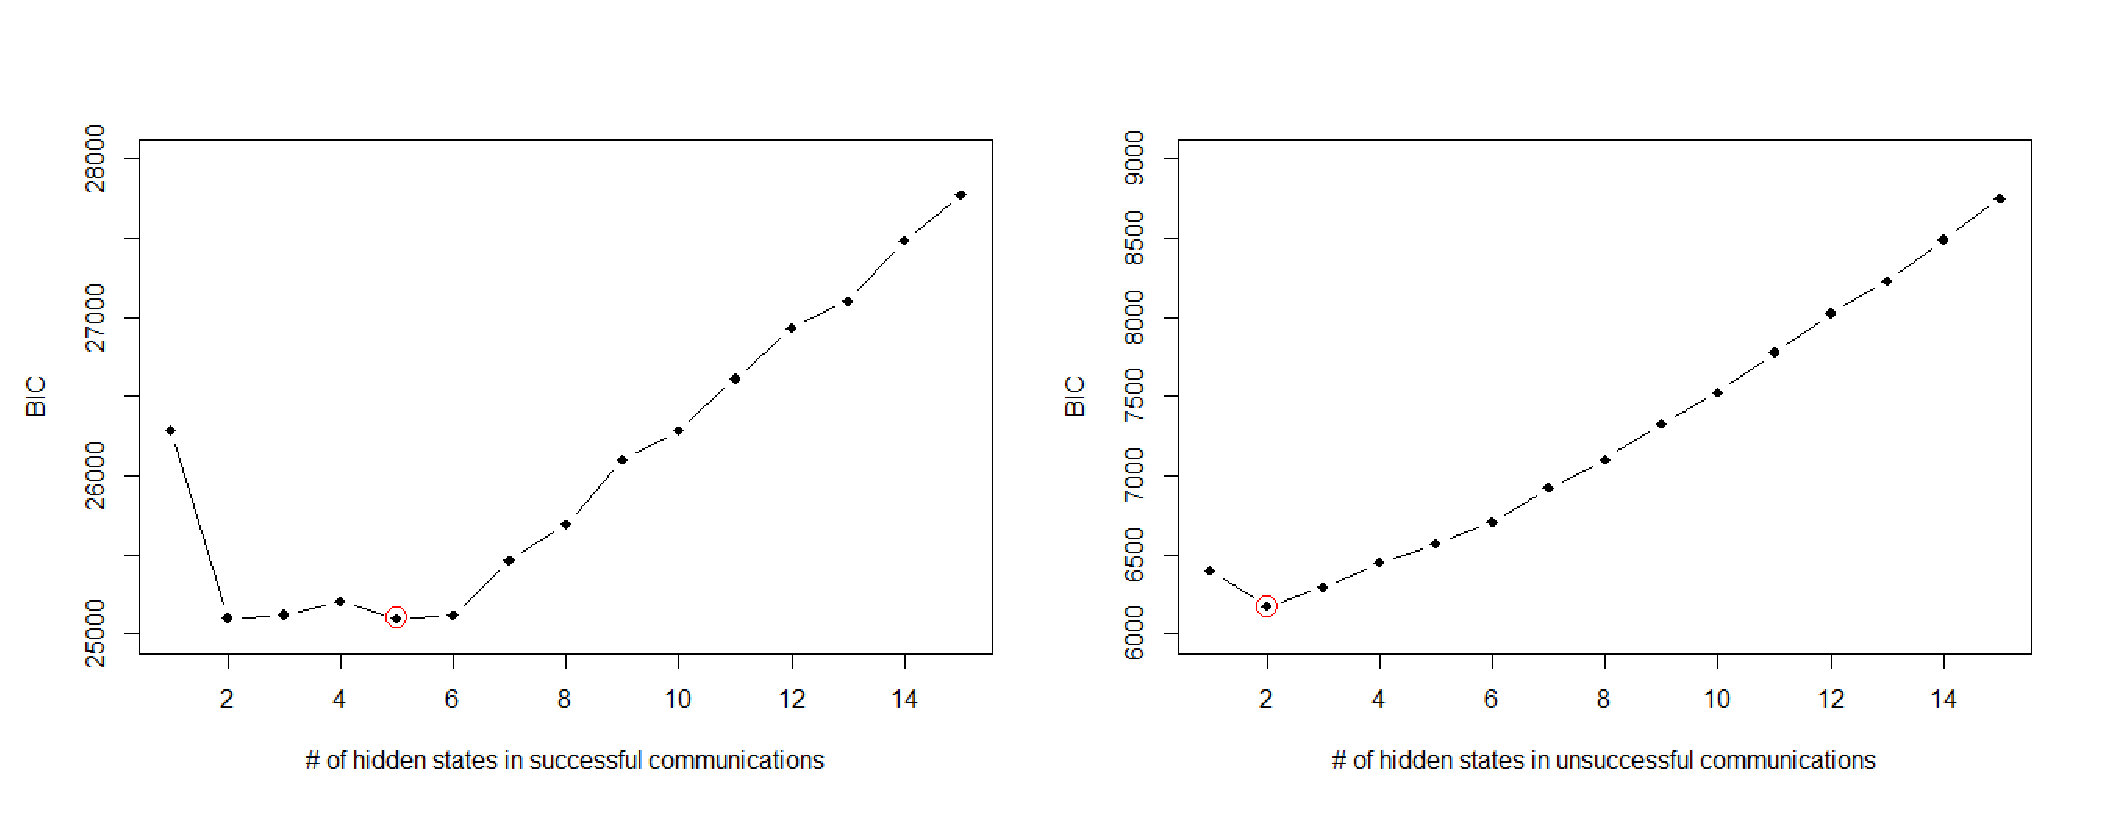
\includegraphics[width=1.0\textwidth]{figures/bic-vs-hidden-states.eps}
\caption{Bayesian information criterion (BIC) of HMM models of successful (left) and unsuccessful (right) interviews by varying the number of hidden states.}
\label{fig:bic}
\end{figure*}

\subsubsection{Frequent Pattern Mining}
\label{subsubsec:frequentPatternMining}
We applied Frequent Pattern Mining to identify frequently occurring patterns of temporally ordered patient-provider behavior codes in successful and unsuccessful communication sequences. Behavior codes in these patterns may be separated by one or more other codes. For this purpose, we utilized FPClose~\cite{grahne2005fast}, an efficient state-of-the-art close frequent pattern mining algorithm implemented in SPMF~\cite{fournier2014spmf, fournier2016spmf}, to identify frequent patterns of patient-counselor communication behaviors in successful and unsuccessful MI communication sequences. SPMF is an open-source library providing more than 150 data mining algorithms. Popular non-close frequent pattern mining algorithms include Apriori~\cite{agrawal1994fast} and FP-Growth~\cite{han2000mining}. A \textit{frequent pattern} is defined as a pattern of temporally ordered observations, which appears in a given set of sequences more often than a user-specified threshold called the minimum \textit{support count}. For example, \{A\}, \{C\}, \{D\}, and \{C, D\} are frequent patterns in the example set of sequences in Figure~\ref{fig:fpm}, since these patterns appear at least 2 times, which is the minimum support count in this example. In this work, we identified and analyzed \textit{closed frequent patterns} among all sequences of behavior codes in successful and unsuccessful communication sequences. A \textit{frequent pattern is closed} if none of its supersets have the same support count~\cite{pasquier1999discovering}, where a set X is a superset of another set Y, if X contains all the elements of the set Y. For example, the itemsets \{A\}, \{C\}, \{D\}, and \{C, D\} in Figure~\ref{fig:fpm} are not closed frequent patterns, since their supersets \{A, B\}, \{B, C\}, \{B, D\}, and \{B, C, D\} have the same support count. Therefore, \{B\}, \{A, B\}, \{A, D\}, \{B, C\}, \{B, D\}, and \{B, C, D\} are closed frequent patterns, since none of their supersets have the same support count. On the other hand, itemsets \{A, C\}, \{A, B, C\}, \{A, B, D\}, \{A, C, D\} and \{A, B, C, D\} have support counts of 1, 0, 1, 0, and 1, respectively, which is less than the minimum support count, and thus are identified as non-frequent itemsets. Since the threshold for minimum support count depends on a task and is typically determined by the domain expert, we follow the procedure in~\cite{moradi2017quantifying, liu1999mining} and set the minimum support count as 10\% of the total number of all communication sequences, which is 110 for successful and 25 for unsuccessful communication sequences. 

\begin{figure*}
\centering
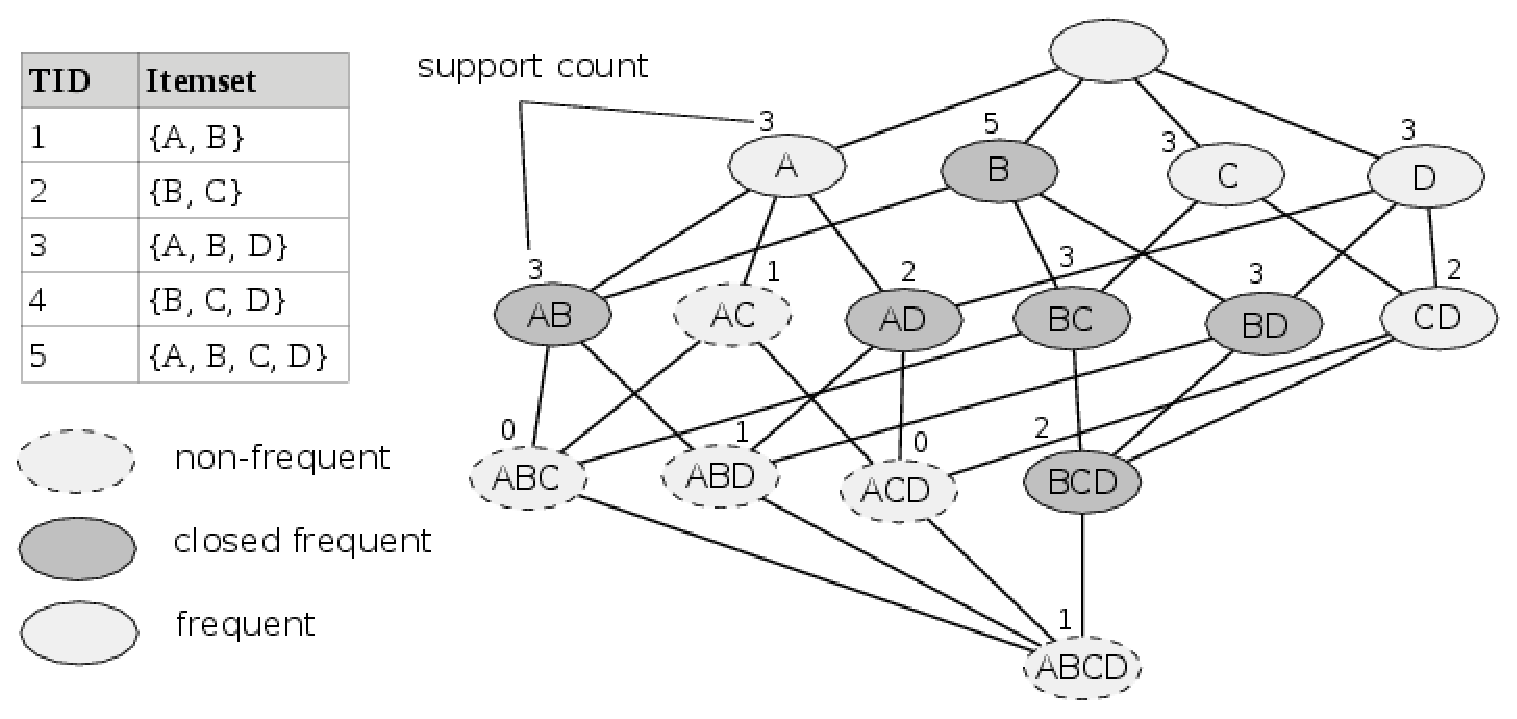
\includegraphics[width=0.8\textwidth]{figures/fpm.eps}
\caption{A sample collection of sequences and different types of frequent patterns obtained by a frequent pattern mining method with the minimum support of 2.}
\label{fig:fpm}
\end{figure*}

\begin{sidewaystable}
\vspace{15\baselineskip}

\caption{Hidden Markov Model Emission Matrices}
\label{tab:emission}
\begin{tabularx}{\textwidth}{lllllllll}
\hline\noalign{\smallskip}
first & second & third & first & second & third & first & second & third  \\
\noalign{\smallskip}\hline\noalign{\smallskip}
number & number & number & number & number & number & number & number & number\\
number & number & number & number & number & number & number & number & number\\
\noalign{\smallskip}\hline
\end{tabularx}

\vspace{2\baselineskip}

\caption{Hidden Markov Model Transition Matrices}
\label{tab:transition}  
\begin{tabularx}{\textwidth}{lll}
\hline\noalign{\smallskip}
first & second & third  \\
\noalign{\smallskip}\hline\noalign{\smallskip}
number & number & number \\
number & number & number \\
\noalign{\smallskip}\hline
\end{tabularx}
\end{sidewaystable}


\section{Results}
\label{sec:results}
The transition and emission probability matrices of HMM model are reported in Tables~\ref{tab:emission} and \ref{tab:transition}. The three behaviors with the highest frequency, representing 45-69\% of each state’s emission probability mass, were used to interpret the emission matrix and label the hidden states. Most (84\%) successful sequences began with a state characterized as \textit{``high motivation''} as evidenced by a greater proportion of three counselor behaviors: reflections of change talk (29\%), reflections of commitment language (17\%), and affirmations (12\%). Successful sequences began with a state of \textit{``high receptivity''} 11\% of the time. \textit{``High receptivity''} sequences were characterized by nearly equal proportions of information offered using patient-centered strategies (18\%), questions to elicit change talk (16\%), and affirmations (15\%). Few successful sequences began in states of \textit{``moderate receptivity''} and \textit{``low receptivity''} (2\% and 3\% of the time, respectively). These two states were characterized by different proportions of the same behaviors. \textit{Moderate receptivity} sequences were distinguished from \textit{low receptivity} sequences by a greater proportion of counselor questions to elicit change talk (20\% versus 11\%) and a lower proportion of patient low uptake statements (16\% versus 28\%); counselor statements emphasizing the patient’s autonomy were about the same (14\% versus 17\%). No (0\%) successful sequence began in the \textit{``active feedback''} state, which was characterized by three patient behaviors, low uptake (47\%), weight-related high uptake (12\%), and other-related high uptake (10\%). Successful sequences transitioned from \textit{``high motivation''} to \textit{``active feedback''} most often (41\%). \textit{``active feedback''}, in turn, most frequently transitioned to \textit{``high receptivity''} (39\%). The \textit{``moderate receptivity''} state transitioned to most often to \textit{``active feedback''} (27\%) and automatically transitioned back to \textit{``moderate receptivity''} (24\%) or to \textit{``low receptivity''} (23\%) with similar frequency. The full transition matrix is presented in Table~\ref{tab:transition}.

In contrast, the majority of unsuccessful sequences (98\%) began in a state of \textit{``ambivalence''} as indicated by the greater proportion of counselor reflections of both change talk (20\%) and sustain talk (12\%) as well as affirmations (13\%). About 2\% of the time unsuccessful sequences started in a state of \textit{``avoidance''}. Higher rates of patient low uptake (29\%) and other-related high uptake (11\%) statements, and counselor patient-centered information (18\%) distinguished \textit{``avoidant''} sequences. Both \textit{``ambivalent''} (84\%) and \textit{``avoidant''} (61\%) states most frequently transitioned to the \textit{``avoidant''} state.

Frequent communication patterns in successful and unsuccessful patient-counselor communication sequences are shown in Table~\ref{tab:patterns}. Results from frequent pattern mining analysis indicate that reflections of change talk were the most frequent counselor communication behavior in both successful (36.1\%) and unsuccessful sequences (33.7\%). For each pattern, the statistical significance of difference between pattern occurrence in successful and unsuccessful communications was reported by computing p-value using Pearson’s chi-square test. Successful sequences were distinguished from unsuccessful sequences by a higher frequency of counselor questions phrased to elicit change talk (30.8\% versus 17.4\%, p<0.0001), statements emphasizing the patient’s decision-making autonomy (28.5\% versus 18.6\%, p=0.0012), questions phrased to elicit commitment language (18.1\% versus 11.6\%, p=0.0118), and reflections of commitment language (20.7\% versus 15.1\%, p= 0.0423). In contrast, unsuccessful sequences were characterized by greater frequency of questions to elicit perceived barriers (14.7\% versus 0\%, p= <0.0001), reflections of sustain talk (27.1\% versus 15.8\%, p=<0.0001), providing information (28.7\% versus 22.1\%, p= 0.0254) and other reflections (11.6\% versus 0\%, p=<0.0001). In 14.0\% of the successful sequences, reflections of change talk were paired with a question phrased to elicit change talk; this pattern did not appear in unsuccessful sequences. In contrast, in 10.5\% of the unsuccessful sequences, reflections of change talk were paired with information; this pattern did not appear in successful sequences.

\begin{table}
\begin{threeparttable}
\caption{Frequent communication patterns in successful and unsuccessful patient-counselor communication sequences.}
\label{tab:patterns}   
\begin{tabularx}{\textwidth}{lll}
\hline\noalign{\smallskip}
first & second & third  \\
\noalign{\smallskip}\hline\noalign{\smallskip}
number & number & number number number number number number \\
number number number number & number number number & number number  number \\
\noalign{\smallskip}\hline
\end{tabularx}
\begin{tablenotes}
      \small
      \item This is where authors provide additional information about the data, including whatever notes are needed.
\end{tablenotes}
\end{threeparttable}
\end{table}

\section{Discussion}
\label{sec:discussion}
In summary, this study applied HMM and frequent pattern mining to test the fundamental hypothesis guiding Motivational Interviewing, which posits that counselors use of ``MI-consistent'' communication strategies (MICO) will lead to patient change talk~\cite{miller2009toward}. Previous studies have empirically linked counselors’ use of MICO to higher rates of patient change talk in first-order Markov Chain models~\cite{moyers2006therapist, moyers2009session, gaume2010counselor}. The present study leveraged data mining methods to provide an even stronger evidence for MI’s fundamental hypothesis by considering longer-term dependencies in the data. Unlike simple first-order Markov chain models, frequent pattern mining considers behavioral antecedents beyond the counselor behavior immediately preceding a patient change talk statement, while HMM is able to identify relations between groups of communication behaviors. The ability of HMM and frequent pattern mining to identify critical patterns in patient-counselor communication sequences advances research in the field of Motivational Interviewing, which has previously relied upon simple Markov chain models~\cite{moyers2006therapist, moyers2009session, gaume2008counsellor, gaume2010counselor, glynn2014change, carcone2013provider, jacques2016building}.

The states identified in HMM model, were given labels to describe the underlying ``state'' of the MI session. These labels were based on the analysis and interpretation of the three behaviors with the highest frequency according to the emission matrix. Three behaviors were chosen since together they represented 45-69\% of the behaviors associated with a given state. These labels make it easier for MI practitioners to gain a deeper understanding of the dynamics of interactions occurring between counselors and patients. 

In both analyses, MICO communication strategies were characteristic of successful sequences (i.e., those resulting in a change talk statement). In HMM, the majority of successful sequences began in the high motivation state, when counselors frequently use reflections of change talk or commitment language as well as affirmations. Other high frequency counselor behaviors observed in successful sequences included statements emphasizing patients’ decision-making autonomy, questions phrased to elicit change talk, and the provision of information using patient-centered strategies. The frequent pattern mining results were similar. Reflections of change talk was the most frequent counselor communication strategy in successful sequences, followed by open questions phrased to elicit change talk, affirmations, statements emphasizing the patient’s decision-making autonomy, and sensitively provided information. Previous studies of MI behavior code sequences, which relied on first-order Markov chain models to analyze communication sequences, have linked patients’ expression of change talk to counselor reflections of change talk,~\cite{moyers2009session, gaume2010counselor, glynn2014change, carcone2013provider, jacques2016building} open questions phrased to elicit change talk,~\cite{moyers2009session, carcone2013provider, jacques2016building}, and statements emphasizing the patient’s decision-making autonomy~\cite{carcone2013provider, jacques2016building}. However, these studies did not find a link between change talk and counselors’ use of affirmations or the provision of information, when examined independently of the MICO index. Thus, the present study is the first to provide empirical evidence for these causal linkages. One reason for this unique finding may be the treatment context, adolescent patients engaged in a voluntary weight loss trial. Adaptations of MI for the health care setting suggest that asking questions, demonstrating active listening through reflections, and the provision of information are critical communication skills for encouraging health-related behavior change~\cite{douaihy2015motivational}. Thus, providing information in a patient-centered manner in the context of health care treatment may be necessary to ensure patients have the requisite knowledge of their health care problem and its treatment. 

The analysis of unsuccessful sequences, i.e., those resulting in a patient sustain talk statement, was typified by a combination of MICO and MI-inconsistent communication strategies (MIIN). Specifically, the majority of unsuccessful sequences in the HMM analysis began in a state of Ambivalence which was characterized by large proportions of counselor reflections of both change talk and sustain talk. Similarly, in the frequent pattern mining analysis of unsuccessful sequences, reflections of change talk and sustain talk were two of the three most frequent counselor behaviors observed. These results are consistent with those of Gaume et al.~\cite{gaume2010counselor} who found both MICO and MIIN were linked to the elicitation of sustain talk in a sample of at-risk young adult drinkers enlisted into the military. Specifically, counselors’ use of simple and complex reflections and ``other MICO'' behaviors (an index of affirmations, statements emphasizing patient control, reframing, and support) were empirically linked to the elicitation of sustain talk; neither open or closed questions were related to the elicitation of sustain talk. Carcone et al.~\cite{carcone2013provider} found counselors’ questions and reflections specifically phrased to elicit patient sustain talk were the counselor behaviors most likely to elicit sustain talk among adolescents engaged in a weight loss trial. In contrast, Moyers et al.~\cite{moyers2009session} found questions about the positive and negative aspects of the target behavior and reflections of sustain talk were empirically linked to the elicitation of sustain talk but MIIN was not. These variable findings provide further support for the need to tailor the communication strategies MI counselors use to the treatment context. 

This study is part of a line of research to develop machine-learning models to annotate (code) and analyze patient-counselor communication patterns. We have previously reported on the development of probabilistic generative models~\cite{kotov2014towards, kotov2015interpretable} and application of novel features for maximum margin and deep learning classifiers~\cite{hasan2016study} with the goal of automated annotation of MI session transcripts. Experiments applying the annotation model to novel datasets are underway to assess the generalizability of the model to more diverse types of clinical encounters (e.g, email coaching to increase fruit and vegetable intake, HIV clinical care visits~\cite{carcone2018using}). We also developed and evaluated probabilistic and deep learning methods for the task of predicting success of motivational interviews at any point during the interview~\cite{hasan2018predicting}. In this study, we present the next phase of this research, the sequential analysis of patient-counselor communication data to identify the counselor communication strategies linked to the elicitation of change talk and sustain talk. Next steps include examining the performance of these models in diverse data sets representing different populations and behavioral problems. We are also experimenting with machine learning methods to segment (parse) the stream of communications in weight loss intervention delivered by email into semantically coherent chunks (phrases, sentences or paragraphs), to which the annotation model can then assign a behavior code. Together, these models form the basis of a complete system to automatically code and analyze patient-counselor interactions. An automated system for behavioral coding and analysis could substantially accelerate the pace of research on the causal mechanisms of Motivational Interviewing and inform both the theory and clinical practice by providing clinicians with information about how to best tailor their communication strategies to different patient populations. 

This study is limited by the use of one dataset composed of 37 Motivational Interviewing transcripts of counseling sessions with African American adolescents in weight loss treatment. Thus, there is a need to replicate these findings with larger and more diverse data samples as the findings may not be representative of communication patterns in other contexts employing the Motivational Interviewing framework. In fact, when interpreted in light of the published literature, the results obtained in these experiments suggest that communication patterns are likely to vary given the treatment context. There are, however, consistencies with previous Motivational Interviewing process studies providing support for the validity of our findings and suggesting some counselor communication strategies may cut across treatment contexts. Next steps for this work include enhancing the performance and utility of machine learning models for sequential analysis by combining transcript annotation with sequential analysis. Another limitation of this work is the fact that successful and unsuccessful sequences were analyzed independently. One implication of this approach is that the utility of a counselor behavior, such as the provision of information, to shift an interaction destined to be unsuccessful to successful one, cannot be determined from these analyses.

\section{Conclusion}
\label{sec:conclusion}
These results add to the growing evidence base examining the mechanisms of effect in Motivational Interviewing using modeling approaches that overcome critical shortcomings of previous methods. While counselors’ use of ``MI-consistent'' communication behaviors has been previously linked to higher rates of change talk in correlational studies~\cite{moyers2006therapist, catley2006adherence, thrasher2006motivational, mccambridge2011fidelity} and simple Markov chain models~\cite{moyers2006therapist, moyers2009session, gaume2010counselor}, the use of HMM and frequent pattern mining analyses improves upon these approaches by considering long-term dependencies in the data. The results of this work suggest a more complex pattern between counselor communication behaviors and patient talk that varies depending on the context in which Motivational Interviewing is being used.  

\section{Conflict of Interest}
\label{sec:conflictofInterest}
On behalf of all authors, the corresponding author states that there is no conflict of interest.

\begin{acknowledgements}
This study was supported by a grant from the National Institutes of Health, NIDDK R21DK108071, Carcone and Kotov, MPIs. We would like to thank the student assistants in the Department of Family Medicine and Public Health Sciences at Wayne State University School of Medicine for their help in developing the training dataset. The authors would like to thank Lisa Todd, JD, MA for her thoughtful feedback and clinical expertise in the interpretation of these data.
\end{acknowledgements}

\bibliographystyle{natbib}       % JHIR format
\bibliography{references}   
\end{document}
